\chapter{Energy measurement}
\label{ch:energy_measurement}

% Depending on your subject, you might need multiple research chapters. Moreover, depending on how the research questions are linked, you may need to answer them one by one and then connect the answers into a final discussion chapter. 

% See Canvas for examples of theses with various approaches to structuring the research content.

%energy of system or program
When doing energy measurements it is important to not only measure the energy consumption of the CPU, but also of the memory and disk \cite{acar2016impact}. You can use a hardware method to measure the energy consumption or use a software method to estimate the energy consumption. Using a hardware method is more accurate, but also more expensive \cite{acar2016impact}. Luckily as a student of the University of Amsterdam (UvA) I have access to the DAS. The DAS is a distributed supercomputer with nodes that have different hardware specifications and some nodes are connected to a PDU, through which we can measure the energy consumption \cite{bal2016medium}. This PDU is from Racktivity and has an accuracy of 1\%.\\

The DAS has a head node where all the users connect to. Here the users can reserve nodes and add jobs to the queue. There are multiple releases of the DAS, currently only DAS-4 and DAS-5 are in use. For measuring the energy we needed to run the programs on a specific set of six nodes on the DAS-5. To retrieve the data from the PDU connected to these six nodes we needed to use the DAS-4 and the \textit{smnpwalk} command. There were two kind of energy measurement values we could retrieve, the current power (Watt) and the energy consumption (kWh) from when the node was plugged-in till now. Both methods have a disadvantage when using it. When using the current power you need to retrieve the power constantly and you loose some accuracy because you don't know what the power does in between two measure points. The method of measuring the energy consumption has the problem of showing a number that is too large, the numbers are in kWh and have three decimal numbers. Thus the lowest decimal shows Watt per hour. We found that for small programs it is not sufficient to only measure in Watt per hour, because of the short run times. We tested this with three programs, a idle program where the only command was sleep, two programs who calculates the 10.000th prime one recursively and one who did this optimized. The results of this test are shown in figure \ref{tab:EMmethod}. Here we see that the difference of 0.001 kWh is a large difference when working with numbers that are of scale 0.005 kWh. There isn't a clear difference between primes optimized and the sleep that takes close to the same amount of seconds as the primes optimized. Because of these results we choose to go with the power measurement method.\\

\begin{table}[h]
\centering
\begin{tabular}{|l|l|l|l|}
\hline
       & \textbf{Idle}      & \textbf{Prime}     & \textbf{PrimeOpt}  \\ \hline
Time   & 8m0.002s  & 7m58.443s & 1m2.394s  \\
Energy & 0.033 kWh & 0.037 kWh & 0.005 kWh \\ \hline
Time   & 1m2.002s  & 7m59.611s & 1m2.220s  \\
Energy & 0.004 kWh & 0.037 kWh & 0.005 kWh \\ \hline
Time   & 1m2.002s  & 7m58.503s & 1m2.235s  \\
Energy & 0.005 kWh & 0.036 kWh & 0.004 kWh \\ \hline
\end{tabular}
\caption{A test done using the energy measurement in kWh with three different programs.}
\label{tab:EMmethod}
\end{table}

When using the power measurement method we get as a result a lot of measure points, where each point has a timestamp and a power value. An example of a measurement and these points are shown in figure \ref{fig:primesOpt}. To calculated the total energy consumed during this program we need to calculate the surface beneath the graph. To do this we calculate the surface between two points and add all surfaces together. When two points do not have the same value we choose the average between the two to use for the surface. When looking at the different nodes we see that they all have a different idle power state. To help compare between the nodes and reduce the difference between the measurement moments we removed the idle state from the energy consumption. To do this we measured the idle state one minute before and after a single run of all the programs. The average power was then calculated and subtracted form every measure point. These calculations resulted in the following formula \ref{eq:surface}.\\

\begin{equation} \label{eq:surface}
    E = \sum (t_{n+1} - t_{n}) * \frac{(p_{n} - p_{idle}) + (p_{n+1} - p_{idle})}{2}
\end{equation}

\begin{figure}[h]
    \centering
    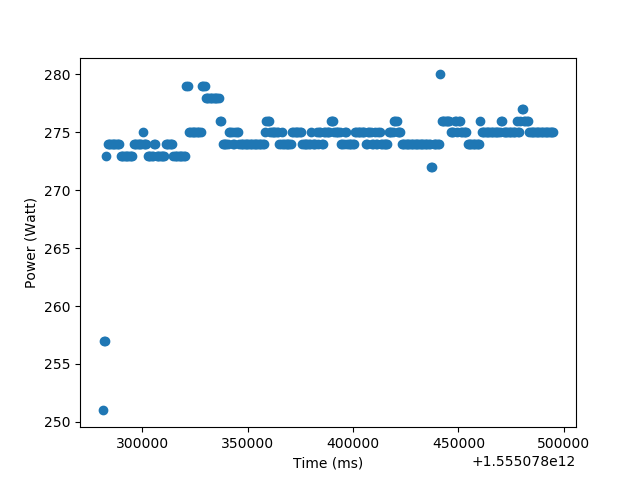
\includegraphics[width=.4\textwidth]{graphs/primesOpt.png}
    \caption{An example measurement of the primesOpt program.}
    \label{fig:primesOpt}
\end{figure}

An overview of the energy measurement set-up can be seen in figure \ref{fig:overview}. Here we can see that from the DAS-5 a job is send to one of the energy measurement nodes. This is done by using the \textit{prun} command and specifying which node to use. The job we send to this node is a bash script that runs all the programs in our data set. In this job we sleep for ten seconds in between the measurements of the programs to give the node time to go back to its idle state. After these ten seconds the measure script on the DAS-4 is started and then the program we want to measure for the energy consumption starts to run on the node. Immediately after the program ends the measure script is stopped. This measure script on the DAS-4 constantly sends a \textit{snmp} message to the PDU and writes the values to an output file. Only six nodes on the DAS-5 are connected to the PDU and all these nodes have different hardware specifications. Therefor we need to separate the measurements to be able to compare the results. Due to the other nodes constantly being occupied, every program was run 27 times on \textit{node28} and 22 times on \textit{node29}. The hardware specifications for \textit{node28} are a GPU node with an Nvidia Tesla K20 (with 6 GB onboard memory), an Xeon Phi and a michost and for \textit{node29} are a GPU node with an Nvidia GTX980 (with 4 GB onboard memory) and an TitanX-Pascal.

% An overview of our set-up can be seen in figure \ref{fig:overview}. On the DAS-5 we have a run script which takes as one of its arguments a filename. This filename is the file we want to test for energy consumption. We run the run script with the command \textit{srun} and choose one of the nodes that is connected to the PDU. The first thing this script does is send a message to the DAS-4 to start the measurement, after this the program which corresponds to the filename is executed and when that is finished the script sends a message to the DAS-4 that the measurement can be stopped. When the DAS-4 receives the message to start measuring it will execute its measure script until it receives the stop message. This measure script constantly retrieves the data from the PDU and writes it to an output file. The files used for this set-up are in a public Git-Hub repository at \url{https://github.com/lukaskoedijk/Green-Software} in the \textit{EnergyMeasurement} folder.

\begin{figure}[h]
    \centering
    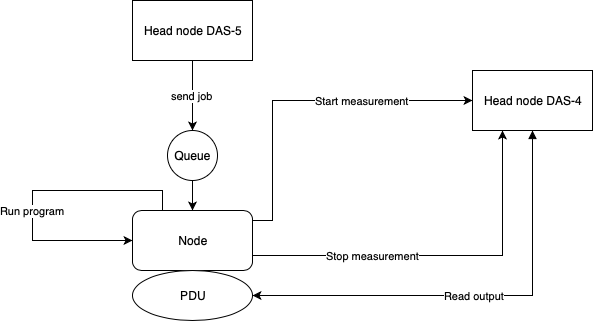
\includegraphics[width=.6\textwidth]{graphs/das.png}
    \caption{The structural overview of how we used the DAS to measure the energy consumption. From the head node of the DAS5 we send jobs to the queue of a certain node we want to measure on. This job will then run on that node when its free. In the job we send a message to the DAS4 to starts its energy measurement, then we run the programs and after that we send a message to the DAS4 to stop the energy measurement. The DAS4 retrieves the energy measurements from the PDU via constant smtp requests.}
    \label{fig:overview}
\end{figure}

The DAS-4 uses \textit{snmpwalk} to retrieve the values form the PDU. The time it takes to retrieve the data from the PDU using \textit{snmpwalk} is not constant. This means that we need to take into account that we have some loss of information and in some cases even too few measure points. When there are less then 30 energy measure points for a program that specific programs will run again until it has enough measure points. In figure \ref{fig:time_diff} the average time between two measure points is shown alongside the standard deviation, the maximum and minimum time difference. There we can see that the average time between two measures is really fast, but the largest time period between two measures is really long. 

\begin{figure}[h]
    \centering
    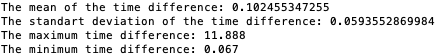
\includegraphics[width=.6\textwidth]{graphs/time_between_measures.png}
    \caption{Some statistics of the time between two energy measurement in seconds.}
    \label{fig:time_diff}
\end{figure}

%-talk about the difference in the nodes (hardware)
%-maybe about measure time diff
%TODO:
%-maybe something about scratch dir, no